\documentclass[11pt,border=5pt]{standalone}
\usepackage{fontspec}
\setmainfont{cmunrm.otf}[BoldFont=cmunbx.otf,ItalicFont=cmunti.otf,BoldItalicFont=cmunbi.otf]
\usepackage{amsmath}
\usepackage{unicode-math}
\setmathfont{NewCMMath-Regular.otf}
\usepackage{tikz}
\usetikzlibrary{arrows.meta,patterns,angles,quotes}
\begin{document}
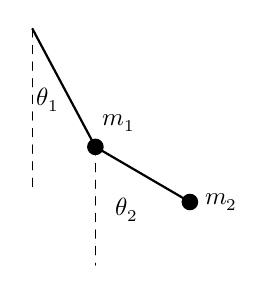
\begin{tikzpicture}[>=Stealth,font=\small,line cap=round,line join=round]
\draw[thick] (0,1.6) -- (0.8,0.1);
\draw[thick] (0.8,0.1) -- (2,-0.6);
\fill (.8,.1) circle (3pt);\fill (2,-.6) circle (3pt);
\draw[dashed] (0,1.6) -- (0,-0.5);
\draw[dashed] (0.8,0.1) -- (0.8,-1.4);
\node at (0.2,0.7) {$\theta_1$};
\node at (1.2,-0.7) {$\theta_2$};
\node at (2.4,-0.6) {$m_2$};
\node at (1.1,0.4) {$m_1$};

\end{tikzpicture}
\end{document}
